\newcommand{\ldshort}[1]{{\bf{[#1]}}\todo{define abbr #1}}
\newcommand{\lcite}[1]{\cite{#1}}
\newcommand{\ignore}[1]

\newduneabbrev{lsst}{LSST}{Large Synoptic Survey Telescope}{8.4 m telescope with 3.2G-pixel camera that will start taking data in 2023.}
\newduneabbrev{ska}{SKA}{Square Kilometer Array}{International radio telescope array planned to start data-taking in 2027.}
\newduneabbrev{hyperk}{HyperK}{Hyper Kamiokande}{260 kT water Cerenkov neutrino detector to begin construction at Kamiokande in 2020.}
% June 17, 2019 - recovered from github 
\newduneabbrev{lhcb}{LHCb}{LHCb}{LHC experiment dedicated to forward physics.}
\newduneabbrev{belleii}{BelleII}{BelleII}{B-factory experiment now running at KEK.}

\chapter{Computing in DUNE}
\label{ch:exec-comp}

%%%%%%%%%%%%%%%%%%%%%%%%%%%%%%%%%%%%%%%%
\section{Executive Summary}
\label{ch:exec-comp-es}

The \dword{dune}  collaboration comprises 178 institutions from 32 countries, including 15 European nations and the \dword{cern}. The experiment is preparing to commission the first 10kT  fiducial mass \dword{lar} \dword{tpc} module between 2024 and 2026 with a long data taking run growing to four modules between 2026 and 2036 and beyond.  An active prototyping program is already in place and has had  a short test beam run in 2018 at \dword{cern}.  These tests used  a 700T, 15,360 channel prototype \dword{tpc} with \dword{sp} readout.  Tests of a \dword{dp} detector of similar size are scheduled for mid-2019.   The \dword{dune} experiment has already  benefited greatly from these initial tests.  The collaboration has recently formed a formal \dword{csc}, with significant participation by European institutions and interest from groups in Asia, to develop common software and computing and to formalize resource contributions.

The consortium resource model benefits from existing \dword{osg}  and \dword{wlcg} infrastructure developed for the \dword{lhc} and broader \dword{hep} community.  \dword{dune}, through  \dword{pdsp}, is already using global resources for simulating and analyzing  \dword{pdsp} data.  Several European institutions are part of this resource pool and are making significant contributions to the \dword{pdsp} and \dword{pddp} programs.  We expect this global computing consortium to grow and evolve as we move towards gathering data from the full \dword{dune} detectors in the 2020s.

The long term \dword{dune} science program should produce raw data volumes similar in scale to the data volumes that current \dword{lhc} Run-2 experiments have already handled successfully.  Baseline predictions for the \dword{dune} data, depending on actual detector performance and noise levels, are $\sim 30$ PB of raw data per year.  These data, with simulations and derived analysis samples, must be available to all collaborating institutions.  We anticipate that institutions worldwide will be both contributors and end-users of storage and CPU resources for \dword{dune}.

%To enable these resource contributions in cooperation with the \dword{lhc} and other communities, we plan to use common computing layers for infrastructure access and common tools to ease integration of facilities with both the \dword{dune} and \dword{lhc} computing ecosystems.  We will use common data storage methodologies to establish large high-availability data lakes worldwide  and to collaborate with the broader HEP community in developing other common tools.


HEP has considerable infrastructure in place for international computing collaboration thanks to the \dword{lhc} program.  Additional large non-\dword{lhc} experiments, including the \dword{lsst}, \dword{belleii}, \dword{ska}, \dword{dune}, and \dword{hyperk},  will enter operation over the next decade and must use and expand upon this model for international cooperation.  Organizing the broader HEP community is formalized through the \dword{hsf} \cite{Alves:2017she}.  The \dword{hsf} is an organization of interested parties working to use the extensive knowledge gained over the past two decades and anticipate the needs experiments will have over the next two decades to develop a sustainable computing landscape for the HEP community.  The \dword{hsf} white papers and roadmaps emphasize common tools and infrastructure as the underpinnings of this landscape.

\dword{dune}'s computing strategy heavily leverages this model of common tools and infrastructure and features data movement and storage, job control and monitoring, accounting, and authentication that both use and contribute to this global community.   \dword{dune} recognizes that other large-scale experiments have similar needs and will encounter similar issues, thus driving worldwide cooperation on common tools as the most cost-effective way to fulfill the scientific missions of the experiments.  Already in the R\&D phases of \dword{dune} computing, \dword{dune} pilot programs use this model.  Most recently in data management and storage, \dword{fermilab}, \dword{cern}, Rutherford Appleton Laboratory, and other academic institutions in the United Kingdom are collaborating on adapting and using the \dword{rucio} data management systems \cite{Barisits:2019fyl}  to serve as the core data management system for \dword{dune}.

Examples of this proto-culture of international collaboration within \dword{dune} were demonstrated during the 2018 test beam run of the \dword{pdsp} detector.  During this run, the \dword{sp} detector at \dword{cern} produced raw data at rates of up to 2GB/s.  These data were transferred and stored in the archive facilities at \dword{cern} and \dword{fermilab} and replicated at sites in the United Kingdom and Czech Republic.  In a more recent commissioning test for the \dword{pddp} detector similar rates have been achieved to CERN/FNAL and the CCIN2P3 computer center in Lyon.

In total, \SI{1.8}{PB} of raw data were produced during the 10 week test beam run, mimicking, within a factor of two, expected data rates and volumes from the initial running of the \dword{fd} complex.  The prototype run was used to examine and test the scalability of existing and proposed computing infrastructure and to establish operational experience within the institutions which have expressed interest in the development and construction of the \dword{dune} computing environment.  Our planning is based heavily on the measurements and information gained from the \dword{protodune} experience.   These measurements are proofs of concept for many of the systems, and their behavior can be extrapolated to the projected levels needed for the full \dword{dune} experiment. 

%The format and organization of \dword{dune}'s data as large multi-dimensional arrays open the possibility of treating the data with computing paradigms similar to those developed for astrophysical image data.  These image processing techniques heavily leverage advances in machine learning and pattern recognition.  Moreover, these techniques benefit from computing resources available at high performance computing (HPC) facilities (supercomputers), where massively parallel and computation heavy algorithms can be mapped onto hardware topologies where they scale better than with traditional batch farms.  Machine learning and HPC oriented analysis is a very active field with continuous advances coming from the current generation of \dword{lar} experiments such as \dword{argoneut}, \dword{microboone}, \dword{sbnd}, and \dword{icarus}.  \dword{dune} is poised to benefit from this work and to expand on it as part of its computing and analysis model.

In summary, \dword{dune}'s computing strategy must be global, working with partners worldwide, and collaborative because almost all computational challenges we face are also those facing similar experiments.  We are extremely fortunate to have the ProtoDUNE tests data to exercise our computing infrastructure and to develop algorithms for  full \dword{dune} operations.
 
%%%%%%%%%%%%%%%%%%%%%%%%%%%%%%%%%%%%%%%%
\section{Computing Consortium}
\subsection{Overview}
\label{ch:exec-comp-ovr}
The mission of the \dword{dune} computing consortium (CSC) is to facilitate the acquisition, processing, and analysis of both detector data and supporting simulations for the \dword{dune} experiment.  This mission must extend over all of primary physics drivers for the experiment and must do so both cost effectively and securely. The \dword{csc} provides the bridge between  online \dword{daq} and monitoring systems and the different physics groups who develop high-level algorithms and analysis techniques to perform measurements with the \dword{dune} data and simulation. The \dword{csc} works with collaborating institutions to identify and provide computational and storage resources.  They provide the software and computing infrastructure in the form of analysis frameworks, data catalogs, data transport systems, database infrastructure, code distribution mechanisms, and other support services essential for recording and analyzing the data and simulations. 

The \dword{csc} works with national agencies and major laboratories to negotiate use and allocation of computing resources.  This work includes support for near term and R\&D efforts like \dword{protodune} runs and extends to the design, development, and deployment of the \dword{dune} computing model and its requisite systems.
These designs include evaluating major software infrastructure systems to determine their usefulness for \dword{dune} physics requirements.   These evaluations should identify opportunities to adopt or adapt existing technologies and engage in collaborative ventures with HEP experiments outside of \dword{dune}. 

At first glance,  the \dword{dune} CPU and storage needs are modest on the scale of the projected rates and needs for the high luminosity \dword{lhc} experiments.  %Initial calculations and extrapolations place the data volumes for the \dword{dune} \dword{fd} program on par with the volumes produced during \dword{lhc} Run-2. 
However, the  beam structure, event sizes, and analysis methodologies make \dword{dune} very unlike collider experiments in event processing needs and projected computational budgets.  In particular, the large \dword{dune} event sizes present a novel technical challenge when data processing and analysis are mapped onto  current and planned computing facilities. In particular, the advent of high performance computing systems optimized for parallel processing of large data arrays presents DUNE with a potential advantage, as our event structure is more suited to those architectures than conventional tracker based HEP data.
Neutrino oscillation analysis and parameter extraction also present novel computational challenges.  

These novel features of \dword{dune} data will require significant effort to adapt to the global computing resources available to the experiment.  These global resources will  likely be both more heterogeneous in computational capabilities (featuring CPU, GPU, and other advanced technologies) and more diverse in topological architectures and provisioning models.  The \dword{dune} computing consortium must address these issues of diversity and architecture to fully exploit the global resources available after 2026 and enable all collaborators to access the data and perform the scientific mission of the experiment.  

%In addition to CPU and storage resources, a substantial core team of computing experts is needed to drive the development of 
novel computing models and manage computing operations in a complex and changing international environment.  

%\section{Consortium Organization}



%%%%%%%%%%%%%%%%%%%%%%%%%%%%%%%%%%%%%%%%
\subsection{Resources and Governance}
\label{ch:exec-comp-gov}

The computing and software group is now a \dword{dune} consortium.  Reference~\cite{bib:docdb12751} describes the governance structure for the consortium.  The consortium coordinates effort across the collaboration, but funding comes from collaborating institutions, laboratories, and national funding agencies. Aside from a small fraction of the consortium leadership \dword{fte}, it is not supported by DUNE or LBNF project funds.  

The consortium has an overall consortium leader. The consortium leader is responsible for the sub-system deliverables and represents the consortium in the overall \dword{dune} collaboration.
In addition, technical leads act as overall project managers for the consortium. The technical leads report to the overall consortium leader.
\dword{csc} has both a Host Laboratory Technical Lead to coordinate between the \dword{dune} project and host laboratory and an External Technical Lead to coordinate with other entities.
At least one of the three leadership roles should be held by a non-US scientist. 
Other roles are currently filled on a voluntary basis by the consortium management.  A more formal structure for institutional contributions and commitments is being constructed. 
%As with other \dword{dune} consortia, the \dword{csc} provisionally divides institutional
%responsibilities for computing resources, deliverables, and operations among the participating institutions.

%This division of responsibilities must account for the resources that are likely to be available. The internally agreed upon division of responsibilities must be presented to the technical board, which will then recommend the collaboration management for approval.

%\todo{Insert Org Chart}

\begin{figure}[htp]
\centering
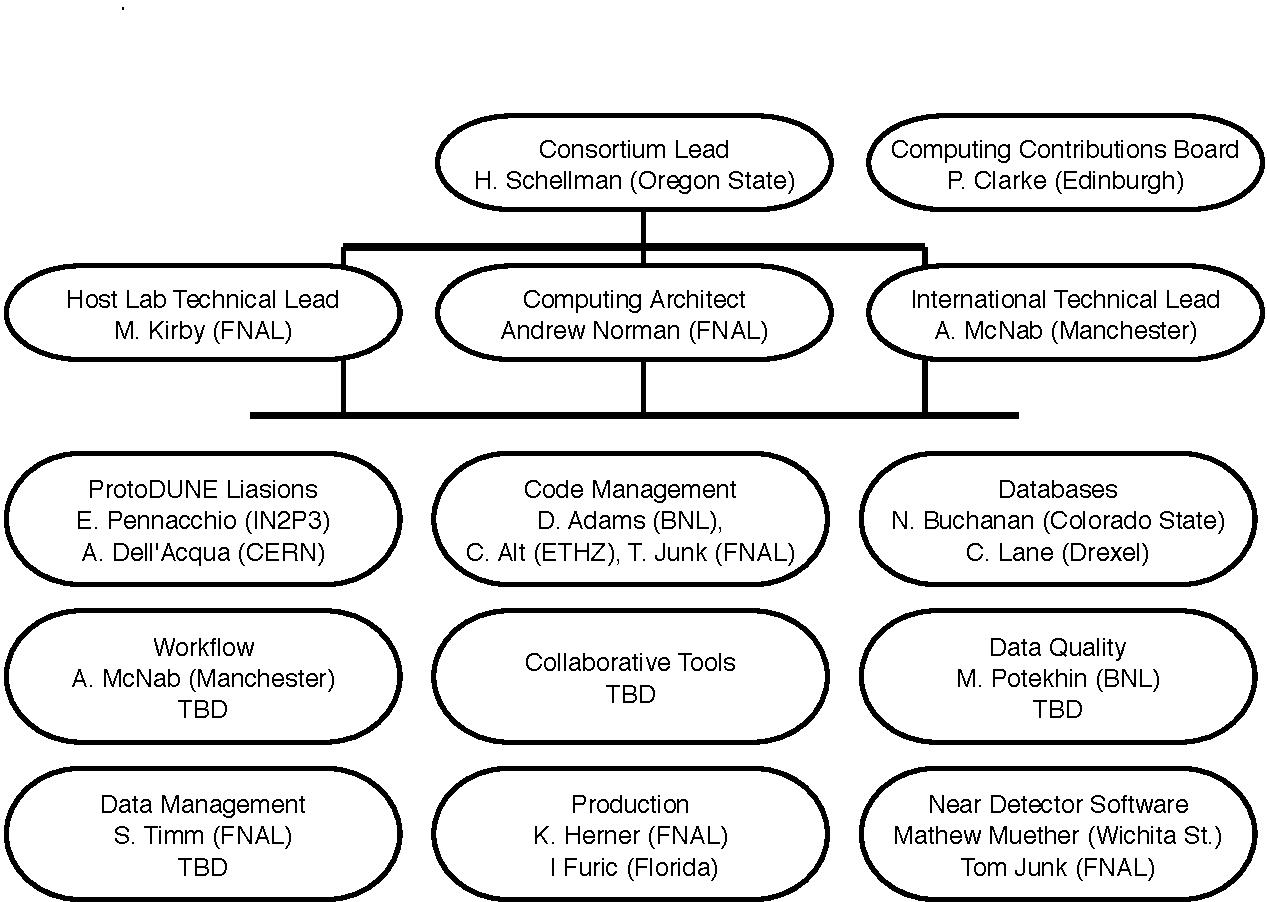
\includegraphics[height=3in]{graphics/comp_Org_Chart.pdf}
\caption{Organization chart for current \dword{csc}. }
\label{fig:ch-exec-comp-org}
\end{figure}

\subsection{Scope of the Consortium}
The \dword{csc}'s focus is the hardware and software infrastructure  for offline computing.  Responsibility for development of algorithms  resides within the physics groups while online systems at experimental sites are governed by the \dword{daq} and \dword{cisc} consortia. The \dword{csc} plays a coordinating role through the definition of interfaces, coding standards and training. All groups coordinate closely to ensure that the full chain of data acquisition, processing, and analysis works. Formal interfaces with the \dword{daq} and controls groups are described in Docdb 7123 (DAQ)\cite{bib:docdb7123} and Docdb 7126 (CISC)\cite{bib:docdb7126}.

The \dword{csc} operates at two levels: at the hardware level, where generic resources can be provided as in-kind contributions to the collaboration, and at the human level, where individuals and groups help develop common software infrastructure.  The   technology for hardware contributions (grid CPU and storage) exists and was exercised during the protoDUNE data run and simulation and reconstruction. Highlights of that effort are discussed below and in the Tools and Methods section of the Physics volume.  



%Thanks to the substantial investment in grid computing infrastructure and storage systems at major laboratories, CPU and long-term storage resources sufficient for development and protoDUNE reconstruction and analysis have come together very well.  However human resources dedicated to DUNE specific projects are still in the formative stages with very little funding as yet identified for full-time personnel. 

\begin{figure}[htp]
\centering
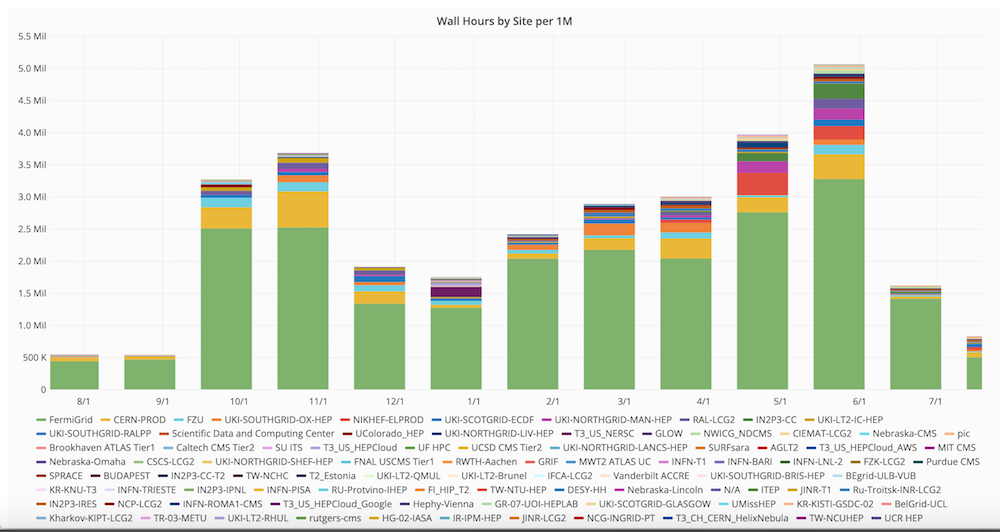
\includegraphics[height=3in]{graphics/comp-ComputingLastYear.png}

\caption{CPU wall-time from July 2018 to July 2019, the 1st peak shows  ProtoDUNE-SP reconstruction while the second is dominated by data analysis and ProtoDUNE-DP simulation. A total of 31 million wall-hours were delivered with 24 M-hrs coming from Fermilab.  }
\label{fig:ch-exec-comp-cpupie}
\end{figure}


\subsection{Hardware Infrastructure}
As illustrated in Figure \ref{fig:ch-exec-comp-cpupie} the \dword{dune} collaboration has already used substantial global resources through the \dword{wlcg} and \dword{osg} mechanisms. As the experiment evolves over the next five years, institutions and collaborating nations will be asked to formally pledge resources (both CPU and storage), and those resources will be accounted for and considered in-kind contributions to the collaboration.  A   computing resources board  is being set up to administer this process and liaise with national resource providers. 

Several international partners are already contributing substantially to CPU resources and we continue to  integrate additional large national facilities. Most CPU resources are opportunistic, but \dword{fermilab} and \dword{cern} have committed several thousand cores and several PB of disk while \dword{dune} has been one of the first beneficiaries of the United Kingdom's IRIS project to provide computing for astronomy and particle physics.  
We are working with \dword{osg} and \dword{wlcg} to integrate reporting mechanisms for CPU utilization so that accurate monitoring of hardware contributions will be in place for the second ProtoDUNE run in 2021-2022 and the buildup to data taking in the mid 2020's. 


\begin{dunetable}
[DUNE CSC members as of July 2019]{lll}{tab:exec-comp-consortium}{DUNE Computing and Software Consortium members as of July 2019.}%-- indicates sites not yet integrated into production computing. }%\rowtitlestyle
Institution& Country \\\colhline%& Integrated\\
KISTI&Korea\\\colhline %&--\\
TIFR  & India \\\colhline%& in process \\
Nikhef&NL\\\colhline%&Yes\\
Edinburgh&UK\\\colhline%&Yes\\
Manchester&UK\\\colhline%&Yes\\
RAL/STFC&UK\\\colhline%&Yes\\
Argonne&USA\\\colhline%&Yes\\
BNL&USA\\\colhline%&Yes\\
Cincinnati&USA\\\colhline%& Yes\\
Colorado State&USA\\\colhline%& Yes\\
CU Boulder&USA\\\colhline%&Yes\\
Fermilab&USA\\\colhline%& Yes \\
Florida &USA\\\colhline%& Yes\\
LBNL&USA\\\colhline%&Yes\\
Minnesota&USA\\\colhline%&Yes\\
Northern Illinois Univ.&USA\\\colhline%&USA& --\\
Notre Dame&USA\\\colhline%&Yes\\
Oregon State University&USA\\\colhline%&Yes\\
Tennessee&USA\\\colhline%&--\\
Texas, Austin&USA\\%&--\\
\end{dunetable}

\subsection{Personnel}

%The \dword{csc} has (or will have) subgroups for the following areas.  Highlights of some of the ongoing projects are detailed in subsequent sections. 

Development of a  dedicated DUNE computing team, responsible for operations and development of new tools specific to DUNE's needs is ongoing. 
%The current DUNE \dword{csc} effort is being done via part time effort by a wide group of contributors from multiple institutions.
Figure \ref{fig:ch-exec-comp-org} shows the current organization.  Very few of these individuals are full time and we largely rely on use of common tools and techniques shared with other, smaller, experiments at CERN and Fermilab. In particular, DUNE currently operates as one of several "Intensity Frontier" experiments at Fermilab, with access to substantial shared resources but very few personnel assigned specifically to DUNE.  As one of our basic design tenets is cooperation and reuse of tools with the broader community, a significant shared component is indeed useful but a small team of dedicated personnel still needs to be built. 
The full DUNE software and computing effort will be much larger in scale and needs to begin serious construction and operations well before commissioning begins at SURF. The unique DUNE data footprint and anticipated evolution in processor technologies will necessitate major efforts to construct and operate the computing infrastructure we will need for the full experiment.

Personnel resources similar in scale to that for \dword{lhcb} and \dword{belleii}, which have a similar collaboration size and international scope, will be needed.  
Much of the high level algorithm development will be done by collaboration scientists but a dedicated core group of experts with strong programming and project management skills will be needed to build and operate the core software infrastructure for the experiment.  We have used the \dword{lhcb} organization structure for a first estimate of our future personnel requirements.

Appendix \ref{comp-roles} describes  computing personnel activities in detail.  In summary, around ten FTE of software development will be needed to develop and maintain the core software necessary to run DUNE algorithms and distributed software infrastructure.  Some of this effort will be shared with other collaborations and \dword{hsf}/\dword{wlcg} projects but in return, DUNE will need to make substantive contributions to those common efforts. In addition, there are specific operational roles such as data manager, code librarian, user support and management that will require personnel dedicated specifically to DUNE computing. Based on \dword{lhcb} experience we have identified ten such roles ranging in FTE from 0.5 to 2.0.  These roles can be filled by experienced DUNE collaborators or computing professionals but should be explicitly recognized as contributions to the experiment. 
\fixme{ Deal with appendix formating}



%\subsection{Work packages}
%The definitions of work packages and assignment to institutions is still being developed. %Different institutions have different competencies and it is important to understand what needs to be done before deciding who will do it.  
The \dword{csc} is instituting a series of workshops, starting with Data Model and Infrastructure in the summer and fall of 2019, to set the scope of subprojects in preparation for a formal TDR. Table \ref{tab:comp-milestones} gives a draft timeline for the computing project.

\begin{dunetable}[Milestones for DUNE Computing Development]{l l r}{tab:comp-milestones}{Milestones for DUNE Computing development.  Data volumes assume 15 PB/year of compressed raw data starting in 2024.}
Year	&	Activity	&	integrated data, PB	\\%
2018	&  	&	10	\\
	& 	ProtoDUNE SP beam run	&	\\
2019	&		&	19	\\%
	&	ProtoDUNE SP processing	&		\\%
	&	ProtoDUNE DP commissioning and data taking	&		\\%
	&	Develop resource model	&		\\%
	&	Develop high level task list	&		\\%
2020	&		&	21	\\%
	&	Continue ProtoDUNE processing/operations	&		\\%
	&	Formalize international resource model	&		\\%
	&	Build operations team	&		\\%
	&	Evaluate data and computing models	&		\\%
	&	Data base design for hardware	&		\\%
2021	&		&	25	\\%
	&	CDR/TDR	&		\\%
	&	Produce Computing TDR	&		\\%
	&	Framework modifications for HPC 	&	\\%	
	&	Data base design for conditions/configuration	&		\\%
2022	&		&	39	\\%
	&	ProtoDUNE second beam run	&		\\%
	&	Begin large scale purchases for FD commissioning	&		\\%
2023	&		&	43	\\%
	&	Reconstruct/analyze protoDUNE results	&		\\%
	&	Continue ProtoDUNE processing/operations	&		\\%
	&	Support FD commissioning	&		\\%
	&	Conditions and configuration data fully integrated	&		\\%
	&	Acquire storage for first year of data from one module	&		\\%
2024	&		&	66	\\%
	&	First real data from 1 FD module	&		\\%
	&	Full operations team in place	&		\\%
	&	Data analysis challenges	&		\\%
2025	&		&	88	\\%
	&	Complete provisioning of hardware/storage for first beam run	&		\\%
2026	&		&	111	\\%
	&	First beam run with 2 modules 	&	 	\\%
	\end{dunetable}
\todo{Need to confirm timeline}

\subsection{Resources contributions}

A formal resource funding model is being developed through the \dword{csc} Resource Board. All \dword{dune} collaborating institutions/countries will be expected to contribute to the computing and software effort.  Contributions will be a mix of CPU resources, storage and personnel with the mix tailored to the resources and capabilities of the institution. To date, these contributions have been voluntary and opportunistic but will evolve to a more formal pledging model similar to that for the LHC experiments.

\section{Data Types and Volumes}

%The DUNE data structure is considerably different from previous neutrino and present collider experiments. Neutrino experiments, including DUNE, run at low rates - of order 1 Hz even for near detectors. But DUNE, due to the large volume and number of channels can generate enormous amounts of data from a single readout.
%This leads to unique new challenges in data storage and reconstruction, even where the data volumes and CPU needs are significantly smaller than those for large collider experiments.  In this section we describe the data volumes and types expected for normal running, calibration and supernova readouts of the far detector. 

% text recovered from the iDR

Offline computing for  \dword{dune} faces new and considerable challenges due to the large scale and diverse physics goals of the experiment.  In particular, the advent of \dword{lar} TPC's with exquisite resolution and sensitivity, combined with enormous physical volumes, creates challenges in acquiring and storing large data volumes and in analyzing and reducing them.  
As a result, the DUNE data structure is considerably different from previous neutrino and present collider experiments. Neutrino experiments, including DUNE, run at low rates - of order 1 Hz even for near detectors. But DUNE, due to the large volume and number of channels can generate enormous amounts of data from a single readout.
This leads to unique new challenges in data storage and reconstruction, even where the total data volumes and CPU needs are significantly smaller than those for large collider experiments.  

In addition, the computing landscape is changing rapidly, with the traditional HEP architecture of individual cores running single-threaded applications being superseded by applications efficiently utilizing multiple processors and perhaps demanding GPUs. At the same time, algorithms for \dword{lar} reconstruction are still in their infancy and developing rapidly.  As a result, we have reason to be optimistic about the future but we are not able to predict it accurately.  The \dword{protodune} single test at CERN in the fall of 2018 has provided a wealth of data that will inform the future evolution of  the \dword{dune} computing models.

In this section we describe the data volumes and types expected for normal running, calibration and supernova readouts of the far detector and the potential for the near detector. 



\subsection{Detectors}

%The  \dword{dune} offline computing challenges can be classified in several ways.  We will start with the different detector/physics configurations that drive the large scale data storage and reconstruction. 
%This discussion leans heavily on the \dword{daq} design described in \voltitlespfd and \voltitledpfd  of the \dword{dune} Technical Proposal

The \dword{dune} experiment will consist of four 10~kT fiducial mass far detector modules located at  the Sanford Underground Research Facility, using either single or dual phase Liquid Argon TPC's, and a near detector at Fermilab.
The proposed  full-size  modules for the far detectors will  have an active volume 12m high, 14.5m wide and 58m long. 

\subsubsection{Single-phase technology data estimates}
 Each  \dword{sp}  module will consist of 
150 alternating vertical cathode and anode planes  spaced 3.5 m apart and operated at 180~kV for a 500~V/cm drift field.  The anode planes are made up of \dword{apa}s which are 6.3~m tall by 2.3~m wide and have 2,560 readout channels each. Each channel is sampled with 12-bit precision every 500 nsec. 
For modules of this size, drift times in the liquid argon are of order 2.5~ms and raw data sizes before compression are of order 6~GB per module per 5.4~ms readout window.  With no triggering and no zero suppression or compression, the raw data volume for four modules would be of order 145~exaB/year. Table \ref{tab:exec-comp-bigpicture} summarizes the relevant parameters for the \dword{sp} technology.


\begin{dunetable}[Useful quantities for computing estimates]{lrr}{tab:exec-comp-bigpicture}
{Useful quantities for computing estimates for single phase readout}%\rowtitlestyle
Quantity&Value&Explanation\\ 
\hline
{\bf Far Detector Beam:}\\ \colhline
Single APA readout &41.5 MB& Uncompressed 5.4 ms\\ \colhline
APAs per module& 150&\\
Full module readout &6.22  GB& Uncompressed 5.4 ms\\ \colhline
Beam rep. rate&\beamreprate&Untriggered\\ \colhline
CPU time/APA&100-200 sec&from MC/ProtoDUNE\\ \colhline
Memory footprint/APA&2 GB&ProtoDUNE experience\\ \colhline
{\bf Supernova:}\\ \colhline
Single channel readout &270 MB& Uncompressed 90 s\\ \colhline
Four module readout& 600 TB& Uncompressed 100 s\\ \colhline
Trigger rate&1  per month&(assumption)\\

\end{dunetable}


\begin{dunefigure}[Figure from volume \todo{pointer to SP DAQ section} Expected physics-related activity
    rates in one FD module]{fig:daq-rates}{Expected physics-related activity
    rates in a single \nominalmodsize module. \label{sec:fd-daq:rates}
}
  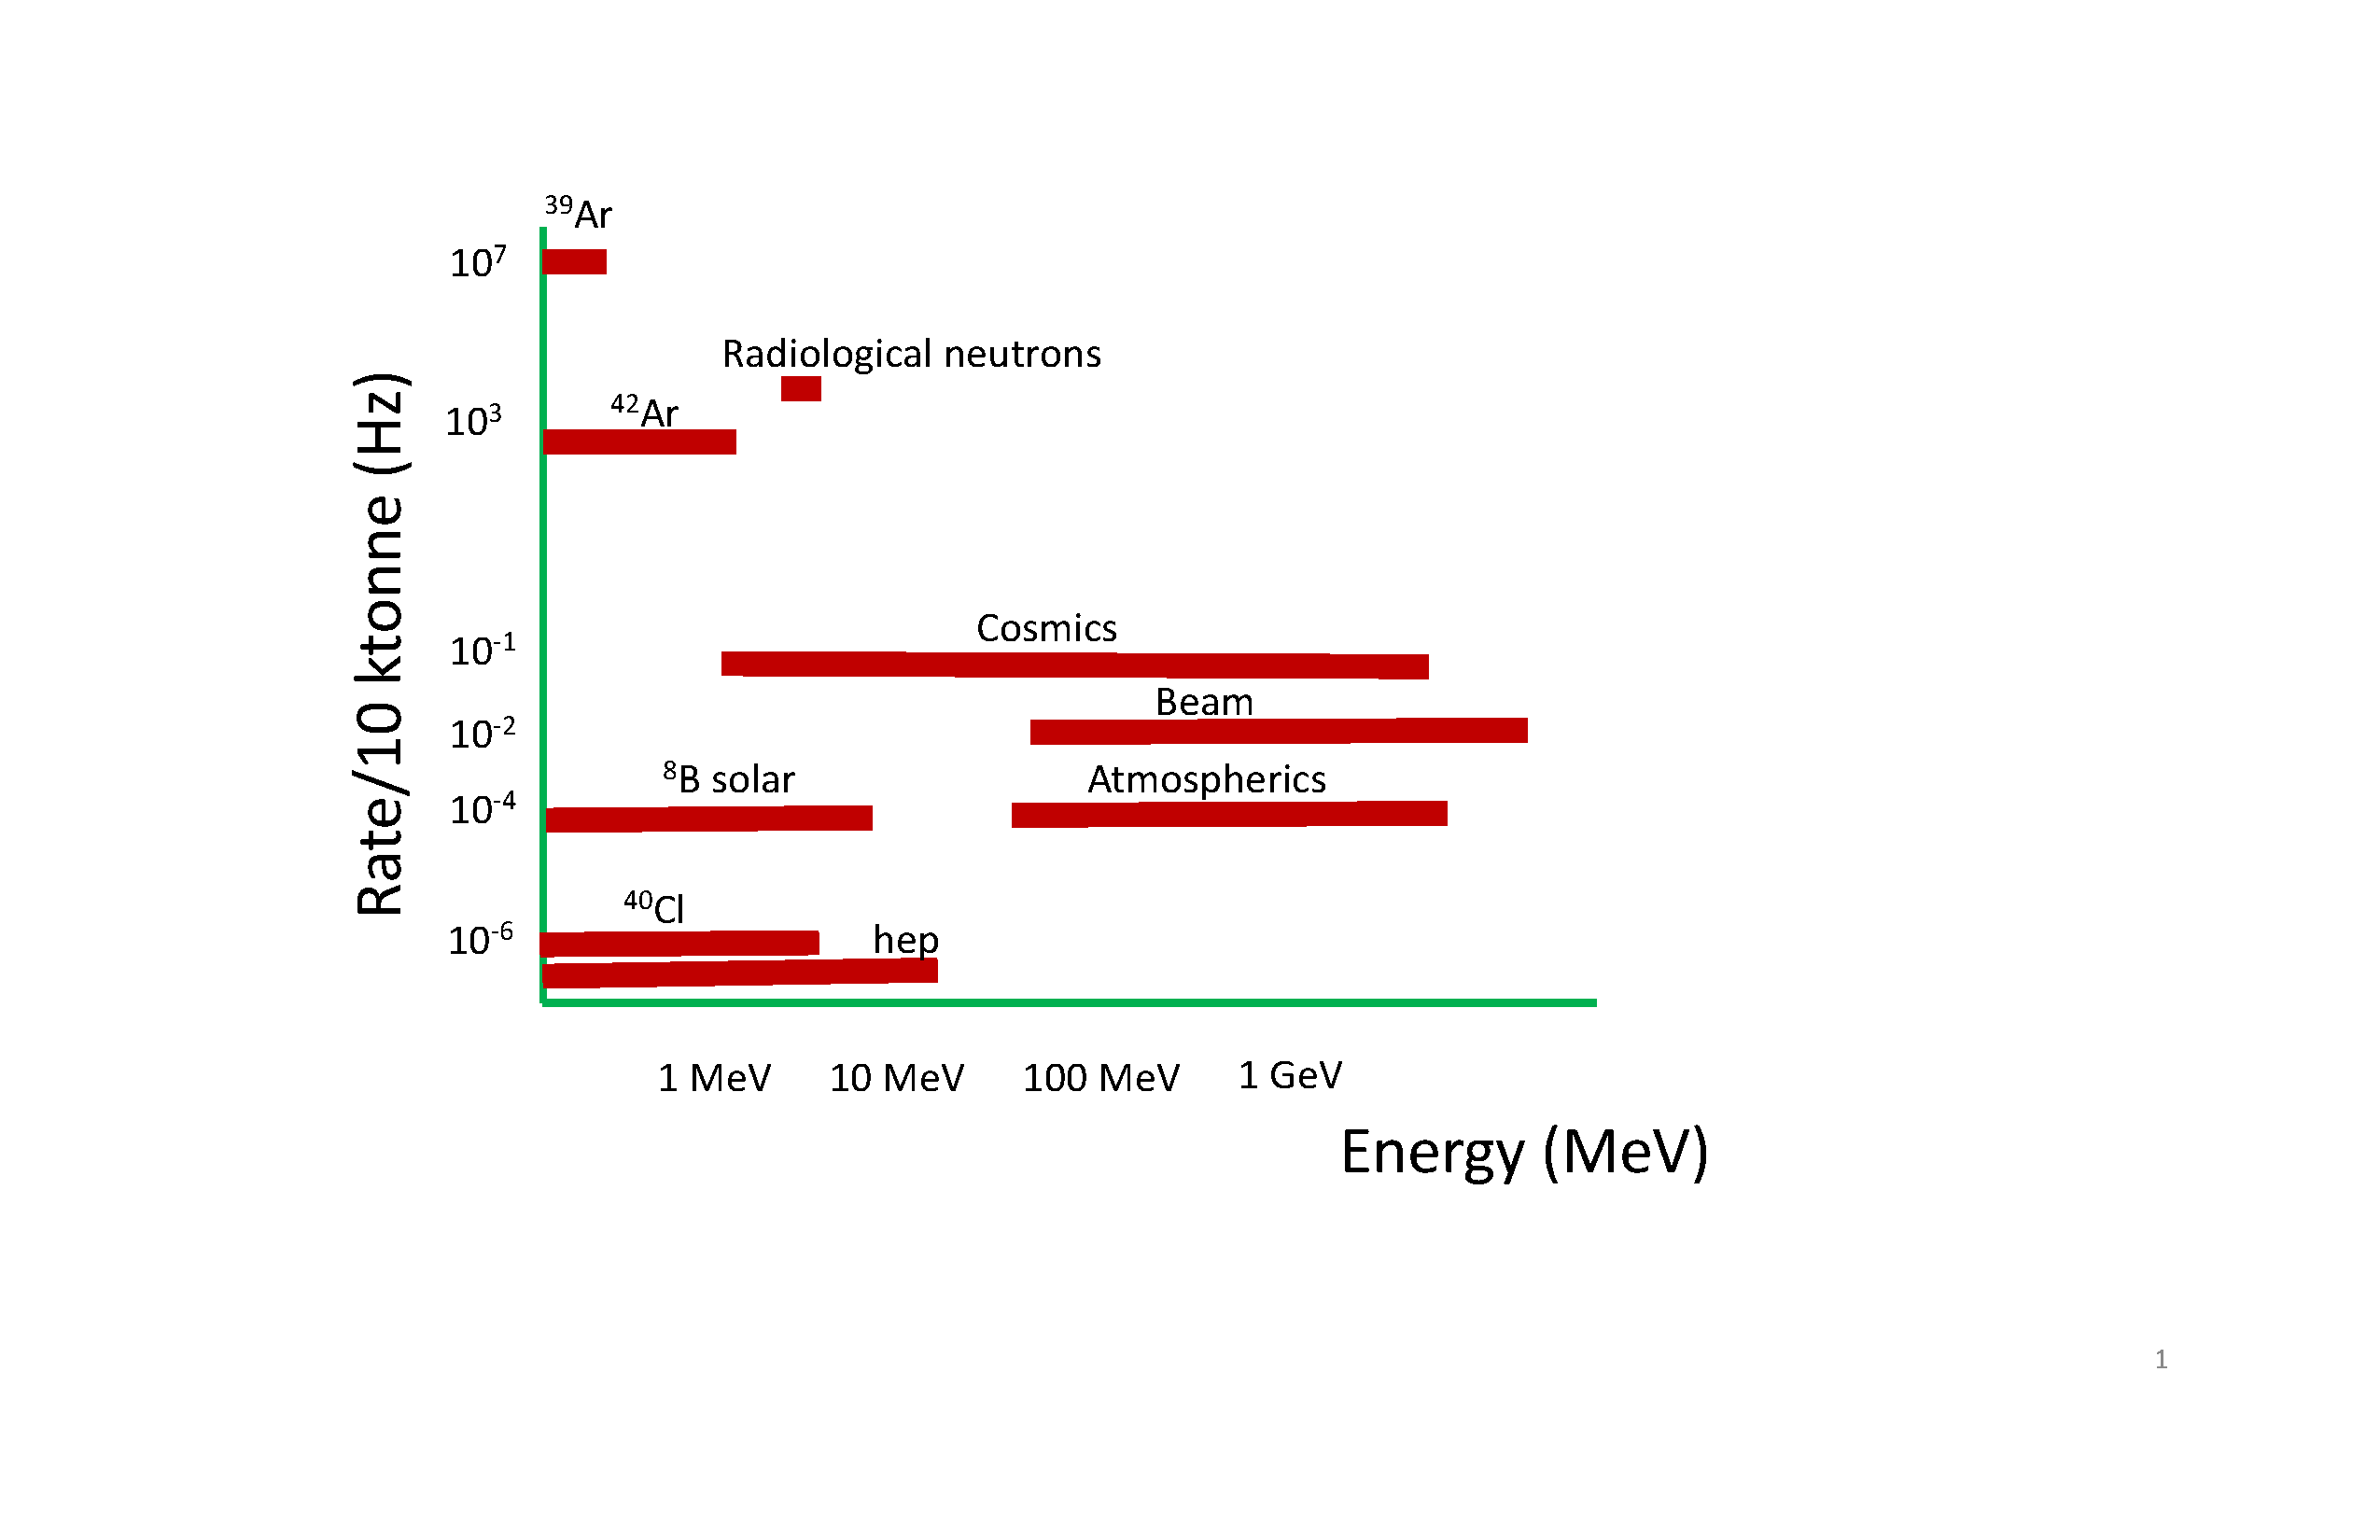
\includegraphics[width=0.7\textwidth,clip,trim=6cm 6cm 10cm 2cm]{daq-event-type-rates-vs-energy.pdf}
\end{dunefigure}

\begin{dunetable}
[Expected DAQ Yearly Data Rates]
{p{0.3\textwidth}p{0.1\textwidth}p{0.5\textwidth}}
{tab:daq-data-rates-sp}
{Summary of expected data rates for initial single-module running with single-phase technology from Volume XXX. The rates assume no compression, and are given for a single \SI{10}{\kilo\tonne} module. Trigger primitives are not kept permanently; they are temporarily stored for 1-2 months at a time. The same applies to fake \dword{snb} data. Improved readout algorithms will be developed and evaluated with the initial data and are expected to provide about an order of magnitude reduction in data while retaining efficiency.}
Source& Annual Data Volume & Assumptions \\ \toprowrule
Beam interactions & 27 TB & 10 MeV threshold in coincidence with beam
time, including cosmic coincidence; \SI{5.4}{\milli\second} readout \\ \colhline
$^{39}$Ar, cosmics and atmospheric neutrinos & 10 PB & \SI{5.4}{\milli\second} readout \\ \colhline
Radiological backgrounds & $<2$ PB & $<1$ per month fake rate for SNB
trigger\\\colhline
Cold electronics calibration & 200 TB & \\ \colhline
Radioactive source calibration & 100 TB & $<10$ Hz source rate; single
APA readout; \SI{5.4}{\milli\second} readout \\\colhline
Laser calibration & 200 TB & 10$^6$ total laser pulses; half the
TPC channels illuminated per pulse; lossy
compression (zero-suppression) on all channels\\\colhline
Random triggers & 60 TB & 45 per day\\\colhline
%$^{39}$Ar decays & \sim 4 PB & \\\colhline
\end{dunetable}



\subsubsection{Dual-phase technology}

For dual-phase, electrons drift the full height of the cryostat, emerge from the liquid and are collected - after gas amplification, on a grid of instrumented pads at the top of the detector.  The WA105 3x1x1 m test of this technology ran successfully in the summer of 2017\cite{Murphy:20170516}. 
Each detector module will have 153,600 channels. Drift time in the liquid argon is 7.5 ms. Given 20,000 samples in an 8~ms readout, the uncompressed event size is 4.2~GB (for 1 drift window).  Due to gas amplification, the signal to noise ratio is quite high, allowing loss-less compression to be applied at the front-end  with a compression factor of ten, bringing the event size/module to 0.42~GB. Recording the entire module drift window can be considered a pessimistic figure, since events are normally contained in smaller detector regions. A  far detector module can be treated as 20 smaller  detectors (with similar number  of readout channels to the prototype currently being constructed at CERN), running in parallel, each one defining a Region of Interest  (\dword{roi}). For beam or cosmic events it is possible to record only the interesting ROI(s) with the compressed size of a single ROI being 22~MB.

\subsection{Data rates}
\subsubsection{Beam coincident rates}

Requiring  coincidence with the \dword{lbnf} beam will reduce the effective live-time from $\sim$1.2 s  to a 5.4~ms (8~ms for DP)  readout window coincident with the 10 microsecond beam spill, leading to an uncompressed data size for beam-coincident events of around 24 GB for four 17~kT single-phase detector modules (and somewhat less for dual-phase); too high to record permanently at full rate.
Only a few thousand true beam interactions in the far detectors are expected each year.  Compression and conservative triggering based on photon detectors and ionization should reduce the data rate from beam interactions by several orders of magnitude without sacrificing efficiency.  Studies discussed in the \dword{daq} section of this proposal indicate that high trigger efficiencies are achievable at an energy threshold of 10 MeV, leading to event rates for beam-initiated  interactions of $\sim 6,400$/year.
Table \ref{tab:daq-data-rates-sp}, adapted from the \dword{daq} section, summarizes the expected uncompressed rates from one single-phase module. 

\subsubsection{ Near detector} The near detector configuration is not yet fully defined  but we do have substantial experience from T2K and  \dword{microboone} at lower energies, and  \dword{minerva} at the  \dword{dune} beam energies on cosmic and beam interactions under similar conditions.  We can expect that a near detector will experience $\sim$ 1 beam interaction/m$^3$/beam pulse and non-negligible rates of cosmic rays. Initial estimates are that zero-suppressed data rates will be of order 10MB/s leading to yearly data volumes less than a PB.  %Reconstructing these complicated events  will be challenging, we can anticipate reconstruction times comparable to those seen in protoDUNE for around 30M events/year. 






\subsubsection{Processes not in synchronization with the beam spill} These include supernova physics, atmospheric neutrinos, proton decay, neutron conversion and solar neutrinos.  These processes are generally at lower energy, making triggering more difficult, and asynchronous, thus requiring an internal or external trigger.  In particular, supernovae signals will consist of a large number of low-energy interactions spread throughout the far detector volume over a time period of 1-100 seconds. Buffering and storing 100 seconds of data would require around 20,000 readout windows, or around 600~TB per 4-module supernova readout.  At a rate of one fake \dword{snb} event/month, this is around 7~PB of uncompressed data per year.  Reconstructing and analyzing these data will require substantial evolution in our software frameworks, which were developed to process small (1-100 MB) events on single processors. This is a major thrust of DUNE's computing R+D for the future. 

\subsubsection{
Calibration}
In addition to physics channels, continuous calibration of the detectors will be necessary.  It is likely that, for the far detectors, calibration samples will  dominate the data volume. Cosmic-ray muons and atmospheric neutrino interactions will provide a substantial sample for energy and position calibration.  Dedicated runs with radioactive sources and laser calibration will also generate substantial and extremely valuable samples. Table \ref{tab:daq-data-rates-sp} includes estimates for the single-phase far detector.   
$^{39}$Ar decays at rates of $\sim$ 1/kg/sec provide a uniform illumination of the detector volume to monitor electron lifetimes. As discussed in the appendices to the Physics volume,  a single 5 ms readout of the full detector would provide 50K decays for study.  A small number of such readouts/day would provide a global monitor of conditions at the 1\% level but measurements sensitive on meter scales will require $10^4$ more data and can become a significant fraction of the calibration data stream. In summary, $^{39}$Ar cosmic ray and atmospheric neutrino signals collected for calibration make up the bulk of the uncompressed \dword{sp} data volume at $\sim$ 10~PB/year per 17~kT module and will dominate the rates from the far detectors.  













\subsubsection{Zero suppression}

The data volumes discussed above are for un-zero-suppressed readout of the full detector. A combination of local triggering, zero-suppression and  efficient lossless compression mechanisms can substantially reduce the final data volume but previous experience in HEP indicates that signal processing must be done carefully and often happens well into data-taking when the data are well understood.  Experience from  \dword{microboone} and the \dword{protodune} experiments will aid us in developing these algorithms but it is likely that they will be applied later in the processing chain for single-phase.  No zero-suppression is planned for dual-phase.

The constrained environment at the Sanford Lab motivates a model where any further data reduction via zero-suppression is done downstream, either on the surface or after delivery to computing facilities at FNAL or elsewhere. This could be analogous to the HLT's used by LHC experiments. The relative optimization of data movement and processing location is an important consideration for the design of both the \dword{daq} and offline computing but the remote location and resource limitations imposed by the underground detector motivate placement of large scale computing resources offsite. 









\subsection{Simulation}
The bulk of data collected with the \dword{fd} is likely to be background, with real beam interaction events in the \dword{fd} numbering in the thousands/year, not millions. Thus, the size of simulation samples may be less than the unprocessed raw data considered above.  Lower energy events are either very rare or can be simulated in sub-volumes of the whole detector.  As a result, while simulation will be important to the experiment, it should not dominate data volume as it does in many experiments.  

However, simulation inputs such as flux files, overlay samples, and shower libraries pose a special problem because they must be distributed to simulation jobs carefully.   Proper simulation requires that these inputs be distributed in unbiased parcels.  This can be technically difficult to do efficiently in a widely distributed environment and will require thoughtful design. 

\subsection{Analysis}

Analysis formats have not yet been fully defined.  We anticipate that most analysis samples will be many times smaller than the raw data.  However, because they are idiosyncratic to particular analyses and even users,  producing and cataloging them will require carefully designed tools and substantial oversight. 
We need a mix of official samples, produced by physics groups and distributed through a common catalog and file transfer mechanisms, as well as small user samples on local disks. 

Final oscillation parameter scans with large number of nuisance parameters can be quite CPU intensive.  The \dword{nova} collaboration's recent physics results required 10's of millions of  HPC CPU hours at the NERSC facility at LBNL. DUNE collaborators used simpler models but the same techniques to generate some of the results presented in the Physics volume. These large-scale analysis projects will require collaboration-wide coordination of resources and will benefit greatly from optimization for specific architectures.

\subsection{Data storage and retention policies}
Some of the samples listed above are extremely valuable and will require conservative retention policies.   Examples include real neutrino and cosmic ray interactions in the far detector, most of the near detector data and any real supernova events.  These data streams may require multiple copies be retained. Calibration samples and, potentially, fake \dword{snb} triggers may be stored temporarily and discarded after processing. 



\subsection{Summary}
In summary, uncompressed data volumes will be dominated by calibration for the far detectors 10-15 PB/year/module and by beam and cosmic ray interactions in the near detectors.  With four \dword{fd} modules but a conservative factor of four for lossless compression a total compressed data volume of 10-15~PB/year for the far detectors is anticipated. Near detector rates are not yet established but likely to be smaller.   
After discussion with the \dword{sp} Trigger/\dword{daq} group, we have requested that they include as upper limits in their design a  maximum data transfer rate from the far detectors to Fermilab of \surffnalbw, which is consistent with projected network bandwidths in the mid 2020's and a limit of 30~PB/year raw data stored to tape.  
%Table \ref{daq:datarates} summarizes the data rates expected from the \dword{daq} section of this proposal. 


\section{ProtoDUNE-SP as an Example}
\label{ch:exec-comp-proto-SP}
The first \dword{protodune} \dword{sp} run at \dword{cern} in late 2018 has already led to a small scale test of the global computing model.  In the following, we will describe the \dword{protodune} data design and the lessons learned from our experience. Much of this carries over into planning for full \dword{fd} operations. 

\subsection{Introduction}

The \dword{pdsp} detector ran at \dword{cern} in the NP04 beamline from September to November of 2018. Since then, studies of cosmic rays have continued. Before that run, several data challenges at high rate validated the data transfer mechanisms. 

\subsection{Data Challenges}

\dword{protodune} performed a series of data challenges, starting in late 2017.  Simulated data were passed through the full chain from the event builder machines to tape storage at \dword{cern} and \dword{fermilab} at rates up to 2 GB/s.  These studies allowed optimizing the network and storage elements well before the start of data taking.
Note that the full \dword{dune} \dword{fd} would, in writing 30 PB/year, produce data at rates similar to  those demonstrated in the 2018 data challenges. While data rates are likely not technically challenging, the integrated data volume from an experiment that is up 99\% of the time over several decades will be. 

\subsection{Commissioning and physics operations}

The first phase of operations was commissioning the detector readout systems while the \dword{lar} reached full purity.  Data were taken with cosmic rays and beam during the commissioning period. Once high \dword{lar} purity had been achieved, physics data were  taken with beam through October and half of November. %Normal trigger rates were approximately 25 Hz, but tests were done at rates up to 100 Hz. 
Since the beam run ended, cosmic-ray data continues to be taken with varying detector conditions, such as modified high voltage and purity and new readout schemes. 

%\subsection{Data Quality Monitoring}

%\todo{DQM}

\subsection{Data Volumes}
The single-phase \dword{protodune} detector comprises a \dword{tpc} with  six \dword{apa}s, \dword{pd}s, and a \dword{crt}. In addition, the np04 beamline is instrumented with hodoscopes and Cerenkov counters to generate beam triggers. Random triggers  were generated at lower rates to collect unbiased cosmic ray information. The data volume from the test beam run was dominated by readout of the \dword{tpc}. % Each \dword{apa} has 2,560 channels and reads out 12 bit \dword{adc} values at 2 MHz. 
The nominal readout window during beam running was  3 ms to match the drift time at the full voltage of 180 kV, which was maintained for most of the run.  The size of the \dword{tpc} data without compression was  138 MB/event, not including headers.  The uncompressed event size including all \dword{tpc} information and \dword{crt} and \dword{pd} data was 170-180 MB. Compression was implemented just before the October beam physics run, reducing the total size per event from around 180 MB to 75 MB.  In total, 8.1 M beam events were written with a total size of 520 TB.  An additional PB of commissioning data and cosmic ray data has also been recorded. 

\ignore{Table \ref{
tab:exec-comp-pd-volumes} summarizes the raw data volumes.

\begin{dunetable}[Data volumes]{lrr}{tab:exec-comp-pd-volumes}{Data volumes  recorded by \dword{pdsp} as of December 2018.}
Type  & Events & Size\\ \rowtitlestyle
Raw Beam&8.08 M& 520 TB \\ \colhline
Raw Cosmics&3.46 M& 271 TB\\ \colhline
Commissioning&3.86 M& 388 TB\\ \colhline
Pre-commissioning&13.89 M&641 TB\\
\end{dunetable}
}

Events were written out in 8 GB raw data files with each containing approximately 100 events. The beam was live for two 4.5 s spills every 32 s beam cycle, and data were taken at  rates up to 50 Hz (typically 25 Hz) leading to compressed \dword{dc} rates of 400-800MB/sec from the detector.  %Each beam cycle could, therefore, produce 1-4  8 GB output files.  
%In earlier runs with uncompressed data, and during an April data challenge, transfer rates up to 2GB/s were demonstrated over substantial periods. 

%Beam was stopped on November 12, but detector cosmic ray studies continue, some with an increased time window of 7.5 ms to collect more complete tracks for each readout.  This raises the compressed event size to around 170 MB.

\ignore{
\subsection{ProtoDUNE-SP Data Streams}
The \dword{pdsp} data consist of multiple sources in addition to the \dword{tpc} data. One of the major challenges for offline computing systems is merging these data streams into a coherent whole for analysis.  Table \ref{tab:exec-comp-pd-sources} lists the data sources used and their granularity. 

\begin{dunetable}[Data sources]{lrr}{tab:exec-comp-pd-sources}{Data sources.  }
Type & indexed by & destination\\ \colhline
TPC  & run/event & event data\\ \colhline
Photon Detector data & run/event & event data\\ \colhline
Cosmic Ray Tagger & run/event & event data\\ \colhline
Beamline devices & timestamp & beam database\\ \colhline
Detector conditions & timestamp & slow controls database\\ \colhline
DAQ configuration & run & files/elisa logbook\\ \colhline
Run quality & run & human generated spreadsheets\\ \colhline
Data quality & run/event/time & Data Quality web application\\ \colhline
File metadata & file & sequential access via metadata file database\\
\end{dunetable}
}
% Information about the detector conditions, \dword{daq} configuration, and run quality is spread across a number of sources and must be collected and then reduced to quantities relevant for offline data analysis.  %For example, the \dword{sc} system logs detector conditions continually.  
% %Offline analysis must know about data with coarser granularity and have algorithms that can use that information.
% A full conditions database transfer mechanism is being developed but was not available during the run.  As a result, other than beamline information, coarse information is currently added to the \dword{sam} file catalog run by run to allow files with given operating conditions to be easily identified and retrieved. %Beam data is stored in the \dword{ifbeam} database and connected to event data via time stamps.

\subsection{Reconstruction of ProtoDUNE-SP data}
Thanks to substantial previous effort by the \dword{35t} prototype, \dword{microboone} and the \dword{lar} \dword{tpc} community, high quality algorithms were already in place to reconstruct the \dword{tpc}  data.  As a result, a first pass reconstruction of the \dword{pdsp} data with beam triggers was completed by early December, less than a month after data taking ended.  Results from that reconstruction are presented in the Methods section of Volume~\volnumberphysics, \voltitlephysics{} with some highlights summarized here. 



\subsection{Data Preparation}

Before pattern recognition, data from the \dword{protodune} detector is
unpacked and copied to a standard format within the art framework based on \dword{root} %ROOT \fixme{ROOT is in the common glossary but without a definition. I have not used the dword because I'm sure it's the same ROOT.} 
objects. 
%The format is also used in detector simulation events.
This reformatted raw data includes the waveform for each channel, consisting of 6,000-15,000,  12-bit, 0.5 $\mu$sec samples. 
The first step in reconstruction is data preparation to
convert each \dword{adc} waveform into a calibrated charge waveform with
signals proportional to charge. At the end of data preparation, hit \dword{roi}s are identified, and the data outside these regions are discarded.  This leads to significant reduction in data size. This process is described more fully in~\cite{bib:docdb12349} and in the Methods section of the Volume~\volnumberphysics, \voltitlephysics{}.% but is summarized here: \fixme{get methods sec ref}
\ignore{
\begin{enumerate}
\item Each waveform is unpacked into integers.
\item Pedestals are determined per event/per channel from the most common \dword{adc} value. 
\item Pedestals and calibrations are applied. %\label{local:ped}
\item Bad channels, sticky bits, and other known hardware problems are corrected or removed.
\item Signal undershoot that creates a long negative tail is removed. 
\item The waveforms  are deconvoluted.  In the first processing, this was done with simple 1D  convolution for a single wire.  A \twod  method of deconvoluting a detailed detector electrostatic field map, originally developed for \dword{microboone}\cite{Adams:2018dra}, is  now available for \dword{protodune} and will be used in the future reconstruction passes.  It properly undoes the long-range induction effects while keeping efficiency high and bias low.  The deconvolution Fourier transforms the waveform, replaces the  bipolar field response function with a unipolar function, applies a low-pass filter to remove high-frequency noise, and then transforms back.

\fixme{One dimensional (1d) and two dimensional (\twod) should be consistent with one another and probably in LATEX code. (Anne says: I just use \twod and \threed from defs for consistency.)}




\item Finally, regions of interest are defined where the signal exceeds a given threshold, and time slices well outside the \dshort{roi} are dropped. These data feed into the reconstruction algorithms for further pattern recognition. %\label{local:roi}
\end{enumerate}
}


Figures~\ref{fig:ch-exec-comp-chtraw} and~\ref{fig:ch-exec-comp-chtroi} illustrate the transformation of \dword{tpc} data  during data preparation. Note that this represents one wire plane for 3 ms.  A full 5.4 ms readout of four 10kT modules would contain a factor of 3,000 more information than this image.

\begin{figure}[t]
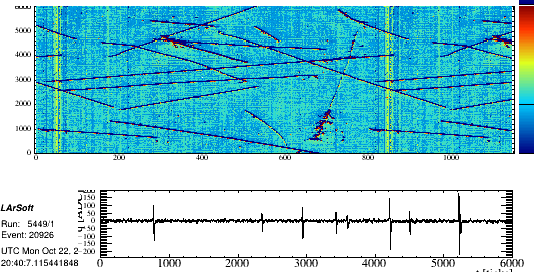
\includegraphics[width=\textwidth,angle=0]{comp-evd_twq-proj_5449_20926_raw.png}
\caption{Example of pedestal-subtracted data for one of the ProtoDUNE  wire planes.  The top pane shows the ADC values in a V (induction) plane with the x-axis being channel number and the y-axis, time slice. The bottom pane shows the bipolar pulses induced on one channel. 
}
\label{fig:ch-exec-comp-chtraw}
\end{figure}

%\fixme{anne commented out includegraphics line because graphic not found - HMS - how did these get lost? THey were there in previous draft - I reloaded them}
\begin{figure}[t]
 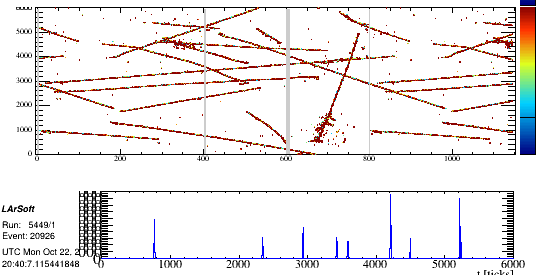
\includegraphics[width=\textwidth]{comp-evd_twq-proj_5449_20926_decon.png}
\caption{
Same as Figure~\ref{fig:ch-exec-comp-chtraw} except after calibration, cleanup, deconvolution and ROI finding. 
}
\label{fig:ch-exec-comp-chtroi}
\end{figure}
%\fixme{anne commented out includegraphics line because graphic not found - it is there in github version}

\subsection{Computational Characteristics of Data Preparation and Deconvolution }
Decoding for \dword{pdsp} was originally done with all six \dword{apa}s in memory. Each \SI{3}{ms} of \dword{apa} readout consists of more than \SI{15}{M} 16-bit values. Decompressing and converting this information to floating point format causes substantial memory expansion. 
  Data with a 7.5 ms window were also taken. 
The input and output event sizes and reconstruction time scale were found to scale linearly with the readout window and with the number of APA's processed. 

%While this helps for protoDUNE,  supernova readout will require additional measures. We are actively pursuing a revised event readout structure which segments the detector in both space and time and modifying the framework to support processing of smaller segments of interaction data. 
Because electrical signals are correlated between channels within an \dword{apa} wire plane but not between planes, processing each wire plane (three per \dword{apa}) independently reduces the memory footprint.
However,  while subdividing the detector into wire planes reduces the memory footprint for short (beam-related) readouts it is  not a viable solution for the long readouts expected for supernova events. We are still exploring the best strategy for dealing with these much larger ($\times 10,000$)time windows. 
%The \dword{daq} group is already testing 1 second ($300 \times$ longer time window) readouts of small numbers of channels.  These are used as tests of optimal models for data segmentation. 
The \dword{daq} consortium is exploring methods for segmenting large events (such as \dword{snb}s) into  smaller of regions of interest in both time and space for efficient readout.  As long as those regions are on the scale of single interactions, the resulting data should fit in a reasonable memory budget at the expense of tracking and collating many distributed interactions. 

The operations performed in signal processing require few decisions but do include operations such as fast-Fourier transforms and deconvolution.  These operations are well suited for GPU and parallel processing. We are actively exploring multi-threaded processing for all data preparation algorithms. 

%\subsection{Further Reconstruction}
%The downstream pattern recognition steps starting with \dword{roi} are described further in %the Tools and Methods chapter of the Physics 
%Volume~\volnumberphysics, Chapter~\ref{}. \fixme{for anne} 

%Table~\ref{tab:comp-raw-data-size} shows the input data size for a typical beam event, dominated by approximately 71 MB of \dword{tpc} waveform information.  
%Table~\ref{tab:comp-reco-data-size} shows the size of different reconstructed objects, still dominated by around 10 MB of reduced \dword{tpc} hit information,  while 
%Table~\ref{tab:comp-reco-data-time} shows the reconstruction time breakdown.  This event had a 3 ms readout window.  
%
\subsection{Reconstruction Characteristics}



Once \dword{roi}s have been identified, several \threed  reconstruction packages are used. For the first reconstruction pass in November, the  \dword{pandora}\cite{Acciarri:2017hat}, \dword{wirecell}\cite{wirecell}, and \dword{pma}\cite{ref:PMA}  frameworks were used with results described in the Physics volume. \fixme{Put in LATEX code.}.  % Table \ref{tab:comp-reco-data-time} indicates that, in terms of CPU time used, these three frameworks are comparable. 
Figure \ref{fig:ch-exec-comp-tracking}  is taken from the from the Physics volume and illustrates the measured efficiency for the Pandora algorithm reconstructing a triggered beam particle as a function of momentum for the simulation and data for selected data taking runs. As can be seen, the efficiency is already quite high and reasonably well simulated.




Full reconstruction of these \dword{pdsp} interactions, with beam particles and approximately 60 cosmic rays per readout window, took of order 600 sec/event with around 200 sec in the signal processing and hit finding stages and the remaining time divided between three different pattern recognition algorithms. Output event records were substantially smaller (22 MB compressed) and still dominated by the information for TPC hits above threshold. 

All of these algorithms are currently being run on conventional UNIX CPU's using \dword{osg}/\dword{wlcg} grid computing  infrastructure. Deep learning techniques based on image pattern recognition algorithms are also being developed. Many of these algorithms can be adapted to run on \dwords{hpc}, although the optimal architecture for \threed reconstruction likely differs from the optimum for hit finding.


\begin{figure}[htp]
\centering
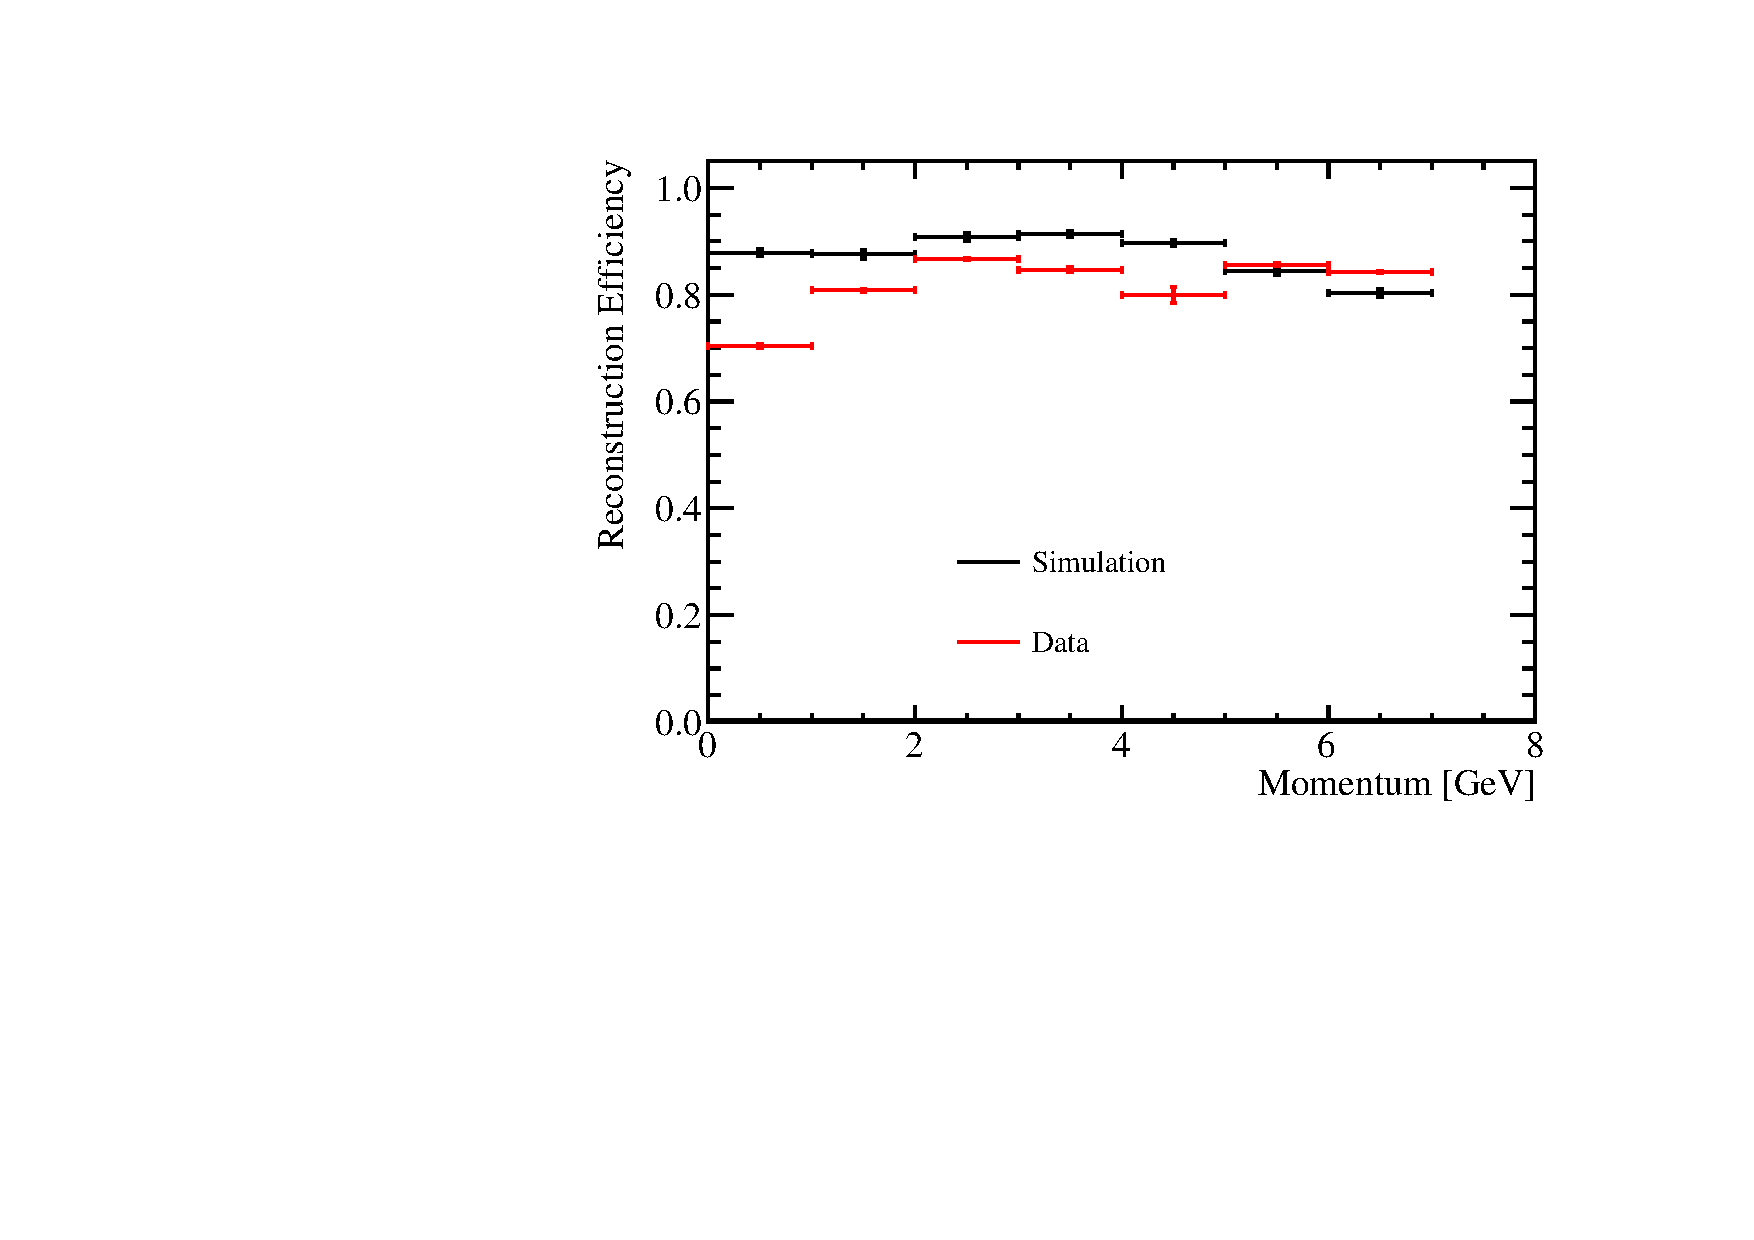
\includegraphics[height=4in]{graphics/BeamParticleEfficiencyVsMomentum.pdf}
\caption{Figure 5.27 from the Physics volume. The efficiency of reconstruction for the triggered test beam particle as a function of particle
momentum in data (red) and simulation (black).}
\label{fig:ch-exec-comp-tracking}
\end{figure}




%\subsection{Processing Infrastructure for Reconstruction and Simulation}
%\label{ch-comp-processing}
%\dword{dune} uses computing resources internationally through the \dword{osg} and \dword{wlcg} infrastructures in the US and Europe.  In 2018, significant effort was put into integrating European sites into the \dword{dune} reconstruction and simulation processing with very positive results.  
%Figure \ref{fig:ch-exec-comp-cpupie} shows the distribution of production jobs worldwide over the past year.  \dword{fermilab} and \dword{cern}, as the host laboratories, contributed the most, but significant resources were also available from the United Kingdom, from the Czech Republic, in Spain and the Netherlands and at IN2P3 in France. %  \fixme{None of the previous abbreviations have been defined in the common glossary. I suspect these should be spelled out or otherwise defined. Unless they are used more than once, I see no point in defining them in the glossary. I do note in the figure (1.3) the abbreviations are used instead of spelling out the terms.}

% \begin{dunetable}
% [Data storage  and CPU needs for reconstruction of ProtoDUNE test beam data]
% {llrrrr}{tab:exec-comp-needs}{Data storage and CPU needs for reconstruction of ProtoDUNE-SP test beam data taken in 2018 and projections for 2019-2021.  We assume two copies of raw data are stored and that each event is reconstructed twice.  Analysis and simulation are estimated to be of order the same CPU use as reconstruction based on the 2018 experience.}%\rowtitlestyle
% \end{dunetable}

%\todo{enter the resource table}

\ignore{
\begin{dunetable}
[Data storage  and CPU needs for reconstruction of ProtoDUNE test beam data]
{llrrrr}{tab:exec-comp-needs}{Data storage and CPU needs for reconstruction of ProtoDUNE-SP test beam data taken in 2018 and projections for 2019-2021.  We assume two copies of raw data are stored and that each event is reconstructed twice.  Analysis and simulation are estimated to be of order the same CPU use as reconstruction based on the 2018 experience.}%\rowtitlestyle
Detector& value &
2018&
2019&
2020&
2021\\\colhline
&&As built\\\colhline
SP&
Events, M&
15.1&
13.0&
6.5&
40.5\\\colhline
&
Raw data, TB&
1047&
2239&
1120&
2799\\\colhline
&
Reco data, TB&
2094&
4479&
2239&
5599\\\colhline
&
CPU, MH&
5.0&
4.3&
2.2&
13.5\\\colhline
DP&
Events, M&
0.0&
101.1&
56.2&
119.9\\\colhline
&
Raw data, TB&
0&
809&
449&
1799\\\colhline
&
Reco data, TB&
0&
1617&
899&
3598\\\colhline
&
CPU, MH&
0.0&
33.7&
18.7&
40.0\\\colhline
total&
Events, M&
15.1&
114.0&
62.6&
160.4\\\colhline
&2x
Raw data, TB&
2094&
6096&
3138&
9197\\\colhline
&
Reco data, TB&
2094&
6096&
3138&
9197\\\colhline
total&Storage, TB&
4188&
12193&
6276&
18394\\\colhline
&
Reco CPU, MH&
5.0&
38.0&
20.9&
53.5\\\colhline
&
Analysis CPU, MH&
5.0&
40.0&
40.0&
40.0\\\colhline
Total&CPU, MH&
10.0&
78.0&
60.9&
93.5\\
\end{dunetable}
}



\subsection{Lessons Learned}
The first protoDUNE run has given us very valuable information for planning the full DUNE computing model. 

\begin{itemize}
    \item Data and simulation challenges led to a reasonably mature and robust model for acquiring, storing, and cataloging the main data stream at design rates.
    \item The experiment integrated several existing grid sites and used substantial opportunistic resources.  This allowed initial processing of data within one month of the end of the run.
    %\item Substantial but successful effort went into signal processing. 
    \item Prototype infrastructure was in place for provisioning; authentication and authorization; data management; networking; file catalog; and workflow management. 
    \item Reconstruction algorithms were available and allowed immediate studies of detector performance and calibration. 
    \item Beam information was successfully integrated into processing through the \dword{ifbeam} database.
    \item Auxiliary information from, for example, slow controls, was not fully integrated into processing which led to  manual input of running conditions by shift personnel and offline incorporation of that information into the data catalog. This has led to closer collaboration with the \dword{daq} and \dword{cisc} groups in designing robust interfaces for configurations and conditions. 
\end{itemize}

Overall, the \dword{pdsp} data taking and processing was a success but overly dependent on doing things manually because automated processes were not always in place. Considerable effort must go into integrating detector conditions, data migration, workflow systems, and \dword{hpc}s with multi-threaded and vectorized software.

%\subsection{Near Future}

%Table~\ref{tab:exec-comp-needs} summarizes known resource usage for 2018 and projections for 2019-2021.  The collaboration has requested a substantial test beam run for both \dword{sp} and \dword{dp} \dwords{detmodule} in 2021-22.  The \dword{csc} views this run as a first production test for the full \dword{dune} computing infrastructure. 





%%%%%%%%%%%%%%%%%%%%%%%%%%%%%%%%%%%%%%%%
\ignore{
\section{Data Model for the Far and Near Detectors}
\label{ch:exec-comp-mod}

%%%%%%%%%%%%%%%%%%%%
\subsection{Introduction}
\label{ch:exec-comp-mod-int}
In parallel with the \dword{pdsp} data, a joint data model task force was formed by the \dword{daq} and \dword{csc} to build a framework for the full \dword{dune} \dword{nd} and \dword{fd}. 
The data model task force grappled with the problems of efficiently triggering, reading out, and storing data on multiple time scales from an enormous detector.

They defined major concepts.
\todo{Request from LBNC to shorten this }

\begin{itemize}

\item{Configuration:} Set of parameters that define the persistent, expected detector state. Globally, this corresponds to a desirable state for the detector, capable of providing data of physics or calibration quality. Each component of the detector may have its own configuration.
 
\item{Run:} Period over which data has been collected across some set of desired components in a consistent configuration.
 
\item{Sub-run:} Period within a run over which data has been collected across some set of desired components in a consistent configuration. The set of desired components in a sub-run must be a subset of the desired components for a run and is the set of components over which data is expected.
 
(Time-based rollovers of runs and sub-runs may be automatic. Differences between sub-run and run due to configuration or changes in the desired components will be tracked by the \dword{daq} and may be either manual or automatic.)
 
\item{Trigger:} Data from the desired components in a sub-run over a readout window. This would typically be centered around a trigger time and is what is recorded by the \dword{daq}. The readout window may be subdivided into frames as determined by the \dword{daq}.
 
\item{Event:} Subset of a trigger isolated in time and space containing an independent interaction in the detector. Events may overlap in space or time within the same trigger. This is generally determined by the offline reconstruction of data in a frame.

\end{itemize}

These definitions are intended to allow triggering, recording, and reconstruction of interactions in subsets of the detector. While the whole detector (or time window) can produce enormous amounts of data, any individual interaction should span a reasonably short time and spatial volume. A data model that can isolate individual interactions  allows interactions to be efficiently stored and reconstructed. 


The main data stream will be augmented by beam, slow controls, \dword{daq} configuration, and calibration information. 

This work continues and informs  the  joint  calibration, \dword{csc} and \dword{daq} designs.

}


\section{Conclusion}

The \dword{dune} \dword{csc} has already undergone a substantial test with the successful run of \dword{pdsp}, including demonstrating data movement to storage at \SI{2}{GB/s}, reconstructing the full test beam sample with high quality algorithms, and beginning analysis of the multiple PB reconstructed data. 

The \dword{csc} is now working with the global HEP computing community to evaluate and specify modern infrastructure that will serve the needs of \dword{dune} and the rest of the community.  We plan to collaborate wherever possible with other experiments where we have common technical challenges. However, the extremely large but simple events generated by \dword{lar} \dwords{tpc}, even with short readouts, present a unique challenge. 

Over the next two years our major activities  will be  thoroughly reviewing available and potential tools, continuing collaborations, and acquiring the resources necessary to launch this large suite of ambitious projects. 


\fixme{Need to make appendices work - may end up deleting them but then need to change reference}

\appendix{Appendix: Computing Roles} \label{comp-roles}

This appendix lists computing roles derived from a comparison with existing \dword{lhcb} roles.  \dword{lhcb} is similar in size and data volumes to \dword{dune}. 

\begin{description}


\item {\bf Distributed Computing Development and Maintenance - 5.0 FTE}
This task includes all software engineering and development activities for packages needed to operate on distributed computing resources. The task requires a good understanding of the distributed computing infrastructure used by DUNE as well as the DUNE computing model.%5.0 FTE

\item {\bf Software and Computing Infrastructure Development and Maintenance - 6.0 FTE}
This task includes software engineering, development and maintenance activities related to central services operated by DUNE to support software and computing activities of the project.   %6.0 FTE

\item {\bf Database Design and Maintenance - 0.5 FTE}
Provides expert assistance to tasks within DUNE which require databases, and helps in addressing performance issues as databases scale. %0.2 FTE

\item {\bf Data Preservation Development - 0.5 FTE}
This task includes activities related to analysis reproducibility and preservation as well as data preservation. The task requires expert knowledge of analysis work and the computing model. %0.5 FTE

\item {\bf Application Managers and Librarians - 2.0 FTE}
Application Managers handle software applications needed for data processing, simulation and analysis. The role includes tasks such as coordination of development activities, release preparation, and the correct deployment of software package releases on software areas needed by DUNE. Librarians organize the overall setup of software packages needed for releases. %The total amount for these roles account for 2 FTE.

\item {\bf Central Services Manager and Operators - 1.5 FTE}
The site manager and operators are responsible for the central infrastructure and services of the DUNE distributed computing infrastructure. This includes liaison with the host laboratory with respect to services they provide for DUNE. %The Site Manager and Operator roles accounts for 1.5 FTE.

\item {\bf Distributed Production Manager - 0.5 FTE}
Distributed Production Managers are responsible for the setup, launch, monitoring and finishing of processing campaigns executed on distributed computing resources of the experiment. Production management is done for data processing, Monte Carlo simulation and working group productions.% The data processing production manager role for all production types accounts for 0.5 FTE.

\item {\bf Distributed Data Manager - 0.5 FTE}
The distributed data manager is responsible for operational interactions with distributed computing disk and tape resources. This role includes activities such as supporting the onboarding of new storage areas, data replication, deletion, movement etc. % The distributed computing data manager role accounts for 0.5 FTE

\item {\bf Distributed Workload Manager - 0.5 FTE}
The distributed workload manager is responsible for operational interactions with distributed computing resources. This role includes activities such as supporting the onboarding of new grid and cloud sites. %The distributed computing workload manager role accounts for 0.5 FTE



\item {\bf Computing Shift Leaders - 1.4 FTE}
The Shift Leader is the main responsible role for distributed computing operations of the experiment. The role is covered by shifts (Monday to Sunday) done by a single person at a time.  They chair the regular operations meetings during their week and attend general DUNE operations meetings as appropriate. %1.4 FTE as it also includes week-ends.

\item {\bf Distributed Computing Resource Contacts - 0.5 FTE}
Distributed computing resource contacts are primary contacts for the DUNE distributed computing operations team and the operators of large (Tier-1) sites and regional federations. They interact directly with the Computing Shift Leaders at operations meetings. %The total of all site contacts accounts for 0.5 FTE and increases with the number of large sites requiring contacts.

\item {\bf User Support - 1.0 FTE}
User support underpins all user activities of the computing project such as software infrastructure, applications and distributed computing, and includes shifts to respond to questions from users on mailing lists and/or Slack-style chat systems and/or ticketing systems, and documenting solutions in knowledge bases and Wikis.% The total FTE count for this role is 1 FTE.

\item {\bf Resource Board chair - 0.1 FTE}
Chairs quarterly meetings of the Computing Resource Board with representatives from the national DUNE collaborations to discuss the level of funding and delivery of the computing resources required for successful processing and exploitation of DUNE data. %0.1 FTE

\item {\bf Computing Coordination - 2.0 FTE}
Overall management of the computing project. %The total amount for this role accounts to 2 FTE.

\todo{Delineate which of these must be dedicated position and which are potentially "shift" duties that can be taken on by individual scientists.   Divide into those two groups.  

May wish to make this an appendix and say that we need around N dedicated full time experts + Y effort from the broader collaboration via shifts or shorter term contributions.
}
\end{description}


% \begin{dunetable}[Core Computing Roles]{l l l}{tab:comp-effort}{Core Computing Roles based on LHCb experience.}
% Role&Details&FTE\\ \colhline
% %Core Software Developers&Software engineering of  core software framework and applications
% %%and libraries & 7.0\\
% %Distributed Computing Software Development&Engineering of frameworks for distributed computing&5.0\\
% %Software and Computing Infrastructure Development and Maintenance&Development and support for distributed computing&6.0\\
% \colhline
% Grid Expert on Call&Primary  responsibility for computing operations&shifts\\
% Distributed Computing Production Managers&Setup, launch, monitoring
% and finishing of processing campaigns& 1.6\\
% Distributed Computing Data Manager&setup of
% storage areas, data replication, deletion, movement&0.6\\
% Distributed Computing Site Contact&Liaisons with major computing sites&many\\
% Application Managers&coordination of development activities, release
% preparation& 1.0\\
% Application Release Manager and Librarian&organize the setup of software packages for release&1.0\\
% User Support & Documentation, training and answering user support questions&1.0\\
% Services \& Operations Managers&Ensure operation of core services, including nightly builds&1.0\\
% Core Developers&Software engineering of  core software frameworks&10\\
% Overall Coordination&Coordinate computing development and operations&2.0 \\
% \end{dunetable}

% \begin{itemize}
%     \item collaborative tools,
% \item data storage and management,
% \item databases,
% \item production and processing, 
% \item workflow management,
% \item \dword{dqm},
% \item software release management, 
% \item core software (led by a software architect),
% \item advanced architectures,
% \item algorithm liaisons, and 
% \item networking.
% \end{itemize}

%%%%%%%%%%%%%%%%%%%%
\appendix{Appendix: Specific collaborative computing projects}
\label{ch:exec-comp-gov-coop}

The \dword{hep} computing community has come together to form a HEP Software Foundation (HSF)\cite{Alves:2017she} that, through working groups, workshops, and white-papers is guiding the next generation of shared \dword{hep} software.  \dword{dune}'s time scale, where we are in the planning and evaluation phase, is almost perfect for us to contribute to and benefit from these efforts.  Our overall strategy for computing infrastructure is to carefully evaluate existing and proposed field-wide solutions, to participate in useful designs, and to build our own solutions only where common solutions do not fit and additional joint development is not feasible.   This section describes some of these common activities. 



\subsection{LArSoft for Event Reconstruction}

The \dword{larsoft}\cite{Snider:2017wjd} reconstruction package is shared by several \dword{lar} neutrino experiments.  \dword{microboone}, \dword{sbnd}, \dword{dune}, and others share in developing a common core software framework customized for each experiment. This software suite and earlier efforts by other experiments made the rapid reconstruction of the \dword{pdsp} data possible.  \dword{dune} will be a major contributor to  the future evolution of this package, in particular, introducing full multi-threading to allow parallel reconstruction of parts of large events, thus anticipating the very large events expected from the full detector. 

\subsection{WLCG/OSG and the HEP Software Foundation}
The  \dword{wlcg}\cite{Bird:2014ctt} organization, which currently combines the resource and infrastructure missions of the \dword{lhc} experiments, has proposed a governance structure that splits dedicated resources for \dword{lhc} experiments from the general middleware infrastructure used to access those resources.  This \dword{sci} is already used by many other experiments worldwide.  In a white paper submitted to the European Strategy Group in December 2018\cite{bib:BirdEUStrategy}, a formal \dword{sci} organization is proposed. As part of the transition to that structure, the \dword{dune} collaboration was provisionally invited to join the \dword{wlcg} Management Board as observers and to participate in the Grid Deployment Board and task forces. The goal of our participation is to contribute to the technical decisions on global computing infrastructure while also contributing to that infrastructure. 
Many of these projecta also involve contributions to and from the broader HEP Software Foundation efforts. 

Areas of collaboration are described in the following. 

\subsubsection{Rucio Development and Extension}

 \dword{rucio}\cite{Barisits:2019fyl}
is a data management system originally developed by the \dword{atlas} collaboration and is now an open-source project.  \dword{dune} has chosen to use \dword{rucio} for large scale data movement.  In the short term, it is combined with the \dword{sam} data catalog used by \dword{fermilab} experiments.  \dword{dune} collaborators at \dword{fermilab} and in the UK are actively collaborating on the \dword{rucio} project, adding value for \dword{dune} but also for the wider effort.


A global \dword{rucio} team now includes \dword{fermilab} and \dword{bnl} staff, \dword{dune}, and \dword{cms} collaborators  in addition to the core developers on \dword{atlas} who initially wrote \dword{rucio}.  Consortium members have started collaborating on several projects:  (a) making object stores (such as Amazon S3 and compatible utilities) work with \dword{rucio} (a large object store in the United Kingdom exists for which \dword{dune} has a sizable allocation);  (b) monitoring  and administering the \dword{rucio} system, leveraging the Landscape system at \dword{fermilab};  (c) designing a  data description engine that can be used to replace the \dword{sam} system we currently use.



\dword{rucio} has already proved a powerful and useful tool for moving defined datasets from point A to point B.  Our initial observation is that \dword{rucio} is a good solution for file localization but is missing the detailed tools for data description and granular dataset definition available in the current \dword{sam} system.  The rapidly varying conditions in the test beam have highlighted a need for a sophisticated data description database interfaced to \dword{rucio}'s location functions. 

In addition,   \dword{lhc} experiments such as \dword{atlas} and \dword{cms} work with disk stores and tape stores that are independent of each other.  This is different from the dCache model used in most \dword{fermilab} experiments where most of dCache is a caching frontend for a tape store.  Efficient integration of caching into the \dword{rucio} model will be an important component for \dword{dune} unless  we can afford to have most data on disk to avoid staging.


%\todo{ Comment on metadata project}

\subsubsection{Testing New Storage Technologies and Interfaces}

The larger \dword{hep} community\cite{Berzano:2018xaa} currently has a \dword{doma} task force
 with which several \dword{dune} collaborators are involved. There are task forces for authorization, caching, third party copy, hierarchical storage, and quality of service. All are of interest to \dword{dune} because they will determine the long term standards for common computing infrastructure in the field. 
In particular, the authorization issues should significantly affect \dword{dune}; they are covered in subsection \ref{ch-comp-auth}.


\subsubsection{Data Management and Retention Policy Development}



A data life cycle is built into the \dword{dune} data model.  Obsolete samples (old simulations and histograms and old commissioning data) need not be maintained indefinitely.  
We are organizing the structure of lower storage, so the various retention types are stored separately for easy deletion when necessary.  

\subsubsection{Authentication and Authorization Security and Interoperability}\label{ch-comp-auth}

Within the next 2-3 years, we expect the global \dword{hep} community to change significantly the methods of authentication and authorization of computing and storage. 
Over that period, \dword{dune} must collaborate with the USA and European \dword{hep} computing communities on improved authentication methods  that will allow secure but transparent access to storage and other resources such as logbooks and code repositories.  The current model, where individuals must be authenticated through different mechanisms for access to USA and European resources, is already a bottleneck to efficiently integrating personnel and storage. 
Current efforts to expand the trust realm between \dword{cern} and \dword{fermilab} should allow a single sign-on for each to access the other laboratory.


\subsection{Evaluations of Other Important Infrastructure}

The \dword{dune} \dword{csc} is still evaluating major infrastructure components, notably databases and workflow management systems.

For databases\cite{Laycock:2019ynk}, the \dword{fermilab} conditions database is used for the first run of \dword{protodune} but the Belle II\cite{Ritter:2018jxh} system supported by \dword{bnl} is being considered for subsequent runs. 

For workflow management, we are evaluating \dword{dirac}\cite{Falabella:2016waj} and plan to investigate PANDA\cite{Megino:2017ywl} to compare with the current GlideInWMS, HT Condor, and POMS solution that has been successfully used for the 2018 \dword{protodune} campaigns.
Both \dword{dirac} and PANDA are used by several \dword{lhc} and non-\dword{lhc} experiments and are already being integrated with \dword{rucio}. 
